\begin{figure}[!t]
	\centering
	\subfloat[Polar coronal hole matching with strong overlap.]
	{
		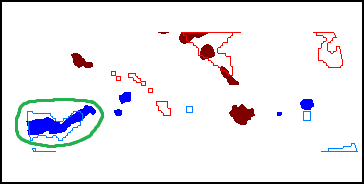
\includegraphics[width=0.45\linewidth]{pictures/thesis/chapter3/matchingProtocol/20100714_m7_matching.png}
		\label{subfig:PtoP_Similar}
	}
	~\subfloat[Polar coronal hole matching with wrap-around effect.]
	{
		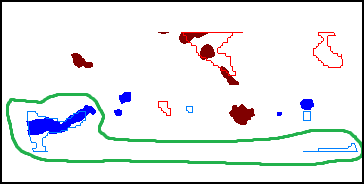
\includegraphics[width=0.45\linewidth]{pictures/thesis/chapter3/matchingProtocol/20100714_m9_matching.png}
		\label{subfig:PtoP_Dissimilar}
	}	

	\subfloat[Mid-latitude matchings with good overlap.]
	{
		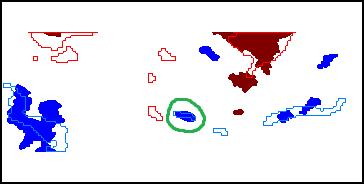
\includegraphics[width=0.45\linewidth]{pictures/thesis/chapter3/matchingProtocol/20110120_m1_matching_mtomSimilar.png}
		\label{subfig:MtoM_Similar}
	}
	~\subfloat[Mid-latitude matching with weak area overlap and
		strong position matching.]
	{
		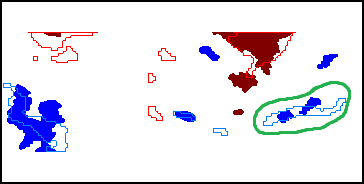
\includegraphics[width=0.45\linewidth]{pictures/thesis/chapter3/matchingProtocol/20110120_m1_matching_mtom_notsimilar.png}
		\label{subfig:MtoM_Dissimilar}
	}
	
	\subfloat[Polar to mid-latitude matching.]
	{
		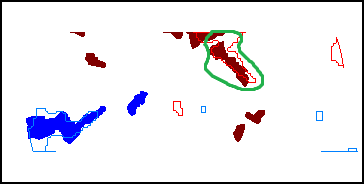
\includegraphics[width=0.45\linewidth]{pictures/thesis/chapter3/matchingProtocol/20100715_m8_matching.png}
		\label{subfig:PtoM}
	}
	~\subfloat[Model generated (new) coronal holes that are not seen
	    in the observations.]
	{
		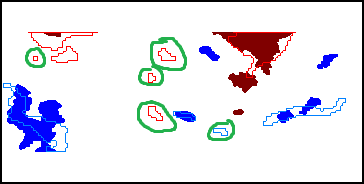
\includegraphics[width=0.45\linewidth]{pictures/thesis/chapter3/matchingProtocol/20110120_m1_matching_gen.png}
		\label{subfig:Gen}
	}
	
	\subfloat[Example showing several coronal holes missing from the observations.]
	{
		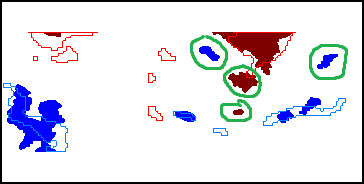
\includegraphics[width=0.45\linewidth]{pictures/thesis/chapter3/matchingProtocol/20110120_m1_matching_rem.png}
		\label{subfig:Rem}
	}
	\caption{\label{fig:matching} 
Coronal hole cluster matching problem. The thick green lines are used for circling out the different matching scenarios. The consensus maps are represented by solid colored coronal hole maps. Negative/positive-polarity coronal holes are depicted as blue/red. The hollow, light-blue/red curves represent the boundaries of the negative/positive-polarity coronal holes derived from the physical models. }
\end{figure}

